\section{Auswertung}

\subsection{Charakteristik des Geiger-Müllerzählrohrs}
\label{sec:charakteristik}

Die gemessenen Daten zur Charakteristik des Geiger-Müllerzählrohrs sind in der Tabelle \ref{tab:ogemessdaten}
angegeben. Dabei ist die Zählrate poissonverteilt und lässt sich gemäß Gleichung \ref{eqn:fehlerzählrate} berechnen.
\newline
Zunächst sollen die Messpunkte mit einem Fehlerbalken in ein Diagramm eingezeichnet werden und anschließend soll entlang des Plateau-Bereiches
eine lineare Ausgleichsgerade erstellt werden. Graphisch lässt sich der Plateau-Bereich, also der Bereich in der die Zählrate kaum zunimmt bei ansteigender angelegter Spannung, grob
als Intervall von $\SI{370}{\volt}$ bis $\SI{630}{\volt}$ festlegen. Durch dieses Intervall kann nun eine lineare Ausgleichsgerade mit folgendem Ansatz gewählt werden.

\begin{equation*}
y = a \cdot x + b
\end{equation*}
wobei $a$ die Steigung der Geraden und $b$ der $y$-Achsenabschnitt ist.
Durch einen linearen Fit lassen sich die Parameter bestimmen zu

\begin{align}
\label{eqn:Param}
a &= \SI{1.138(241)}{{\text{Imp}}\per(\volt\cdot{60}\second)} \\
\label{eqn:Param2}
b &= \SI{9590.735(121824)}{{\text{Imp}}\per{60}\second}
\end{align}

\begin{flushleft}
Die Messwerte mit Fehlerbalken sowie die ermittelte Ausgleichsgerade sind in dem Diagramm
\ref{fig:plot1} dargestellt.

Die Plateau-Steigerung in $\si{\percent\per{100}\volt}$ kann nun durch die zwei Spannungsendpunkte des Plateau-Bereichs $U_{370}$ und $U_{630}$
bestimmt werden. Dazu werden die zugehörigen Zählraten $N_{370}$ und $N_{630}$ über die gefundenen Parameter der
Geraden \eqref{eqn:Param} bestimmt. Da allerdings die prozentuale Steigerung in $\si{\percent\per{100}\volt}$ gefragt ist muss durch den Faktor $2{,}6$ geteilt
werden, da

\begin{equation*}
\frac{\SI{630}{\volt} - \SI{370}{\volt}}{\SI{100}{\volt}} = 2{,}6
\end{equation*}

Für die Prozentuale Steigung $a_{\si{\percent}}$ gilt somit

\begin{equation}
a_{\si{\percent}} = \frac{100}{2{,}6} \cdot\left( \frac{a \cdot U_{630} + b - a \cdot U_{370} - b}{a \cdot U_{630} + b} \right) \si{\percent\per{100}\volt}
\end{equation}

Da die Messwerte allerdings fehlerbehaftet sind gilt die Gaußsche Fehlerfortpflanzung. Dadurch lässt sich
ein $\increment a_{\si{\percent}}$ folgendermaßen bestimmen.

\begin{align}
\increment a_{\si{\percent}} &= \sqrt{\left(\frac{\symup{d}a_{\si{\percent}}}{\symup{d}a}\right)^{2} \cdot 
(\increment a)^{2} + \left(\frac{\symup{d}a_{\si{\percent}}}{\symup{d}b}\right)^{2} \cdot
(\increment b)^{2}} \\
\increment a_{\si{\percent}} &= \frac{100}{2{,}6}\sqrt{\left(\frac{b(U_{630}-U_{370})}{(a \cdot U_{630} + b)^{2}}\right)^{2} \cdot 
(\increment a)^{2} + 
\left(\frac{a(U_{370}-U_{630})}{(a \cdot U_{630} + b)^{2}}\right)^{2}
(\increment b)^{2}}
\end{align}

Nach dem Einsetzen der Werte aus \eqref{eqn:Param} und \eqref{eqn:Param2} sowie den Spannungen $U_{370} = \SI{370}{\volt}$ und $U_{630} = \SI{630}{\volt}$ 
findet sich die prozentuale Steigerung $a_{\si{\percent}}$ auf dem gesamten Plateu-Bereich zu

%\begin{table}
%\centering
%\caption{Zählraten und Fehler.}
%\label{tab:ogemessdaten2}
%\begin{tabular}{c c c c}
%    \toprule
%    Parameter $a$[$si{{\text{Imp}}\per(\volt\cdot{60}\second)}$] & Parameter $b$[$\si{{\text{Imp}}\per{60}\second}$] & Fehler $\increment a$[$si{{\text{Imp}}\per(\volt\cdot{60}\second)}$] & Fehler $\increment b$[$\si{{\text{Imp}}\per{60}\second}$]\\
%    \midrule
%    370   & 1{,}138 & 100{,}20\\
%    630	  & 9590{,}735 & 101{,}11\\
%    \bottomrule
%\end{tabular}
%\end{table}

\begin{equation}
a_{\si{\percent}} = \SI{1.104(218)}{\percent\per{100}\volt}
\end{equation}

%\begin{equation}
%
%\end{equation}

\end{flushleft}
\begin{figure}[h]
  \centering
  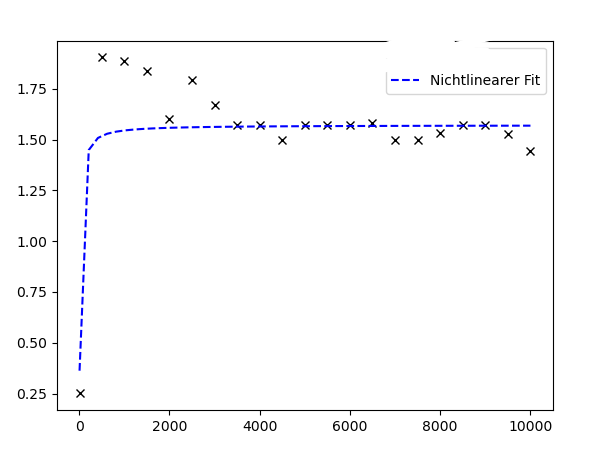
\includegraphics[width=\textwidth]{build/plot1.pdf}
  \caption{Messdaten und Fehlerbalken der Geiger-Müller Charakteristik}
  \label{fig:plot1}
\end{figure}

\subsection{Bestimmung der Totzeit}

\subsubsection{Ablesen am Oszilloskop}
Bei der Versuchsdurchführung wurde am Oszilloskop folgendes abgebildet (siehe Abbildung \ref{fig:abb4}).
Anhand dieser Abbildung lässt sich die Totzeit durch den Abstand zwischen dem ersten zu erkennenden Minimum und dem Minimum der Nachentladung dahinter 
feststellen. Hierbei wurde das Oszilloskop auf $\SI{100}{\micro\second\per{\text{DIV}}}$ gestellt.
Die Totzeit lässt sich grob ablesen zu

\begin{equation*}
T_{tot} \approx \SI{80}{\micro\second}
\end{equation*}

\begin{figure}[h]
  \centering
  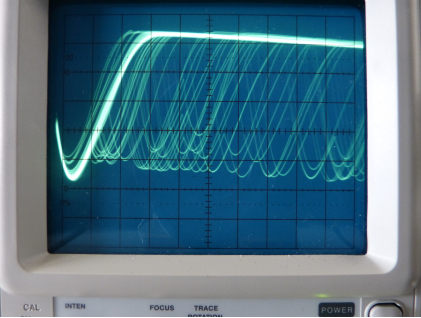
\includegraphics[width=0.65\textwidth]{bilder/Abbildung4.png}
  \caption{Spannungsimpulse am Oszilloskop \cite{ap031}.}
  \label{fig:abb4}
\end{figure}


\subsubsection{Zwei-Quellen-Methode}
Durch die Zwei-Quellen-Methode lässt sich die Totzeit $T_{tot}$ des verwendeten Zählrohrs mit Gleichung \eqref{eqn:totzeit} bestimmen.
Zusammen mit der Fehlerbehaftung der Messwerte nach der Poissonverteilung \eqref{eqn:fehlerzählrate} lässt sich nun wieder eine
Gaußsche Fehlerfortpflanzung formulieren.

\begin{align*}
\increment T_{tot} &= \sqrt{\left( \frac{\symup{d}T_{tot}}{\symup{d}N_{1}}\right)^{2} (\increment N_{1})^{2}
+\left( \frac{\symup{d}T_{tot}}{\symup{d}N_{2}}\right)^{2} (\increment N_{2})^{2}
+\left( \frac{\symup{d}T_{tot}}{\symup{d}N_{1+2}}\right)^{2} (\increment N_{1+2})^{2}
} \\[1em]
\increment T_{tot} &= \sqrt{\left( \frac{N_{1+2} - N_{2}}{2 N_{1}^{2} N_{2}}\right)^2 \cdot N_{1} 
+\left( \frac{N_{1+2} - N_{1}}{2 N_{2}^{2} N_{1}}\right)^2 \cdot N_{2}
+\left( \frac{1}{2 N_{1} N_{2}}\right)^2 \cdot N_{1+2}} 
\end{align*}

Hier werden die Werte aus der Tabelle \ref{tab:ogemessdaten3} verwendet und vor dem Einsetzen auf $\text{Imp} / \si{\second}$ umgerechnet.
Für die Totzeit $T_{tot}$ ergibt sich nach der Zwei-Quellen-Methode folglich

\begin{equation}
T_{tot} \approx \SI{115(47)}{\micro\second}
\end{equation}

\subsection{Bestimmung der pro Teilchen freigesetzten Ladung}

Es gilt nach Beziehung \eqref{eqn:teilchen} ein reziproker Zusammenhang zwischen der freigesetzten Ladung pro eingefallenem Teilchen $Z$ und der
Zählrate $N$ . Bei der Versuchsdurchführung wurde bei der Änderung der Spannung um jeweils $\increment U = \SI{50}{\volt}$ der Zählrohrstrom $I$ gemessen, sowie die Zählrate
$N$ in $\text{Imp}$/$60\si{\second}$. Nun kann die Anzahl der pro Teilchen freigesetzten Ladungen $Z$ aus den gemessenen Werten in Tabelle \ref{tab:ogemessdaten2} bestimmt und anschließend
in Abhängigkeit von der Spannung graphisch dargestellt werden.
\newline
\\
Es gilt wie zuvor der Fehler auf die einzelnen Zählraten $N$ gemäß $\sqrt{N}$ und der angegebene Fehler der Strommessungen in Tabelle \ref{tab:ogemessdaten2} von $\SI{5}{\micro\ampere}$.
Mit der Elementarladung

\begin{equation*}
e = \SI{1.6022e-19}{\coulomb}
\end{equation*}
\begin{flushleft}
folgen dann die Werte für $Z$ nach Umrechnung der Einheiten in das SI-System und einsetzen in die Gleichung 
\eqref{eqn:teilchen}
\end{flushleft}
\begin{table}
\centering
\caption{Ergebnisse der pro Teilchen freigesetzten Ladung $Z$.}
\label{tab:result}
\begin{tabular}{c c c c}
    \toprule
    Spannung $U$[$\si{\volt}$] & Zählrate $N$[$\text{Imp}$/$\si{\second}$] & Stromstärke $I$[$\si{\ampere}$] & Anzahl $Z$ \\
    \midrule
    350  & $\SI{163.95(1280)}{}$ & $\SI{0.30(5)e-6}{}$  & $\SI{1.14(21)e10}{}$\\
    400	 & $\SI{166.58(1290)}{}$ & $\SI{0.40(5)e-6}{}$  & $\SI{1.50(22)e10}{}$\\
    450	 & $\SI{171.06(1308)}{}$ & $\SI{0.70(5)e-6}{}$  & $\SI{2.55(27)e10}{}$\\
    500	 & $\SI{169.18(1300)}{}$ & $\SI{0.80(5)e-6}{}$  & $\SI{2.95(29)e10}{}$\\
    550	 & $\SI{169.73(1303)}{}$ & $\SI{1.00(5)e-6}{}$  & $\SI{3.68(34)e10}{}$\\
    600	 & $\SI{170.88(1307)}{}$ & $\SI{1.30(5)e-6}{}$  & $\SI{4.70(40)e10}{}$\\
    650	 & $\SI{174.88(1322)}{}$ & $\SI{1.40(5)e-6}{}$  & $\SI{5.00(40)e10}{}$\\
    700	 & $\SI{192.45(1387)}{}$ & $\SI{1.80(5)e-6}{}$  & $\SI{5.80(50)e10}{}$\\
    \bottomrule
\end{tabular}
\end{table}

Der Fehler für $Z$ lässt sich wieder durch eine Gaußsche Fehlerfortpflanzung bestimmen.

\begin{align*}
\increment Z &= \sqrt{\left( \frac{\symup{d}Z}{\symup{d}I} \right)^{2} \cdot (\increment I)^{2} 
+ \left( \frac{\symup{d}Z}{\symup{d}N} \right)^{2} \cdot (\increment N)^{2}
}\\
\increment Z &=\sqrt{\left( \frac{1}{e N} \right)^{2} \cdot (\increment I)^{2} 
+ \left( \frac{I}{e N^{2}} \right)^{2} \cdot (\increment N)^{2}
}
\end{align*}
\begin{flushleft}
Abschließend können die ermittelten Werte in Äbhängigkeit von der Spannung $U$ graphisch aufgezeichnet werden.
Dies ist in der Abbildung \ref{fig:plot2} dargestellt.
\end{flushleft}
\begin{figure}[h]
  \centering
  \includegraphics[width=\textwidth]{build/plot2.pdf}
  \caption{Anzahl der pro Teilchen freigesetzten Ladung in Abhängigkeit der Spannung.}
  \label{fig:plot2}
\end{figure}